\chapter{Implementació}

La implementació del joc s'ha realitzar amb dos grans blocs: el servidor i l'interficie client. El servidor es l'encarregat de gestionar la informació realtiva a les partides disponibles, els jugadors conectats i tota la lògica referent a les partides. La interifice client s'encarrega de interaccionar amb el servidor i mostrar la informació al usuari. 

Per l'intercanvi de dades entre el servidor i el client s'utilitzen websockets\footnote{Veure Capítol \ref{sec:websockets}}, ja que ens proporcionen un canal de comunicació bi-direccional a través del protocol HTTP. Aquesta comunicació es totalment asincrona i està basada en events. Així cada vegada que el servidor envía un missatge al client (o a l'inversa) es produeix un event al destinatari i s'executa el codi asociat per al procesament d'aquest events (en cas que n'hi haigi). 

\section{Servidor}

El servidor s'encarrega de les següents tasques: 

\begin{itemize}
\item{Proporcionar un servidor web encarregat de servir el programa client per a cada connexió.}
\item{Emmagatzemar les partides en curs i jugadors connectats. Proporcionar events a través de Websockets per a que els usuaris puguin interaccionar a través del programa client. }
\item{Applicar les regles de la botifarra a cada joc en curs i interactuar amb els diferents clients conectats a una partida}
\end{itemize}

En les properes seccions s'explica més profundament com s'ha realitzat la implementació de cadascuna de les tasques. 

\subsection{Servidor Web}

El servidor web és el proces més important de tot el projecte, ja que és l'encarregat de servir les altres parts de tot el porjecte. 

Per la implementació del servidor web s'ha utiltizat el packet express\footnote{\url{http://expressjs.com/}}. Aquest paquet ens permet desenvolupar servidors web a amb poques línies de codi. Així també disposa de codi pre-programat per tal de realitzar tasques comunes a tots el servidors web. Alguns exemples en són:

\begin{itemize}
\item{Registre de peticions.}
\item{Servir fitxers estàtics (imatges,css,js,etc.).}
\item{Gestió d'errors}
\item{Gestió de galetes (Cookies).}
\end{itemize}

A part de totes aquests funcionalitats, express també s'integra amb diferents llenguatges de plantilles per simplificar l'escriptura del codi HTML. Alguns exemples de motors de plantilles soportats per express són: 

\begin{description}
\item[Haml] {Implementació de Haml\footnote{\url{http://haml-lang.com/}} }
\item[Jade] {Succesor de haml}
\item[EJS] {JavaScript Incrustat}
\item[CoffeeKup] {Plantilles basades amb CoffeeScript}
\item[jQuery Templates for node]
\end{description}

Per la implementació del projecte s'ha utilitzat el motor de plantiles Jade, ja que ens permeten una gran simplificació del codi HTML.

La conjunció de tots els elements comentats anteriorment ens permeten disposar d'un servidor web sobre node.js. Això vol dir que les peticions es procesen de forma asíncrona. 

\subsection{Interconnexió Jugadors}

A part de funcionar com a servidor web el servidor també ha d'intercanviar dades amb els clients conectats amb ells. Per això el servidor crear un WebSocket i proporionar els mecanismes suficients per a que el client s'hi conecti. Així, quan es carrega la primera pàgina de la partida també es carrega el programa client i aquest es conecta al servidor. 

A través de la comunicació amb websockets el servidor es poden realitzar les següent accions: 

\begin{description}
\item[login] {Identificar-se amb el servidor.}
\item[create-game] {Crear una nova partida}
\item[join-game] {Entrar a una partida existent.}
\item[watch-game] {Mirar una partida existent.}
\item[add-bot] {Afegir un robot a una partida existent.}
\item[list-games] {Obtenir una llista de totes les partides disponibles al servidor.}
\item[list-players] {Obtenir una llista de tots els jugadors que hi ha al servidor.}
\item[send] {Enviar un missatge a tota la resta d'usuaris del servidor. }
\end{description}

Cada programa client que es vulgui implementar ha d'utilitzar la comunicació amb WebSockets a través d'aquests events per interactuar amb l'usuari que vol jugar al servidor. Així la comunicació amb WebSockets permet que es pugin implementar més d'un programa client sense tenir que fer cap tipus de modificació al programa servidor. 

\subsection{Lògica Botifarra}

El servidor també és l'encarregat de controlar tot el flux de treball de la botifarra. A la figura \ref{fig:buti-workflow} es pot veure una representació del flux de treball d'una partida de la botifarra, desde que es crea la partida, fins que aquesta es finalitzada. En aquesta figura s'indica amb color blau les funcions que realitzar el programa servidor i amb color verd les que ha de realitzar el propi jugador que està conectat a la partida. 

\begin{figure}[htbp]
\hspace*{-1.5in}
\centering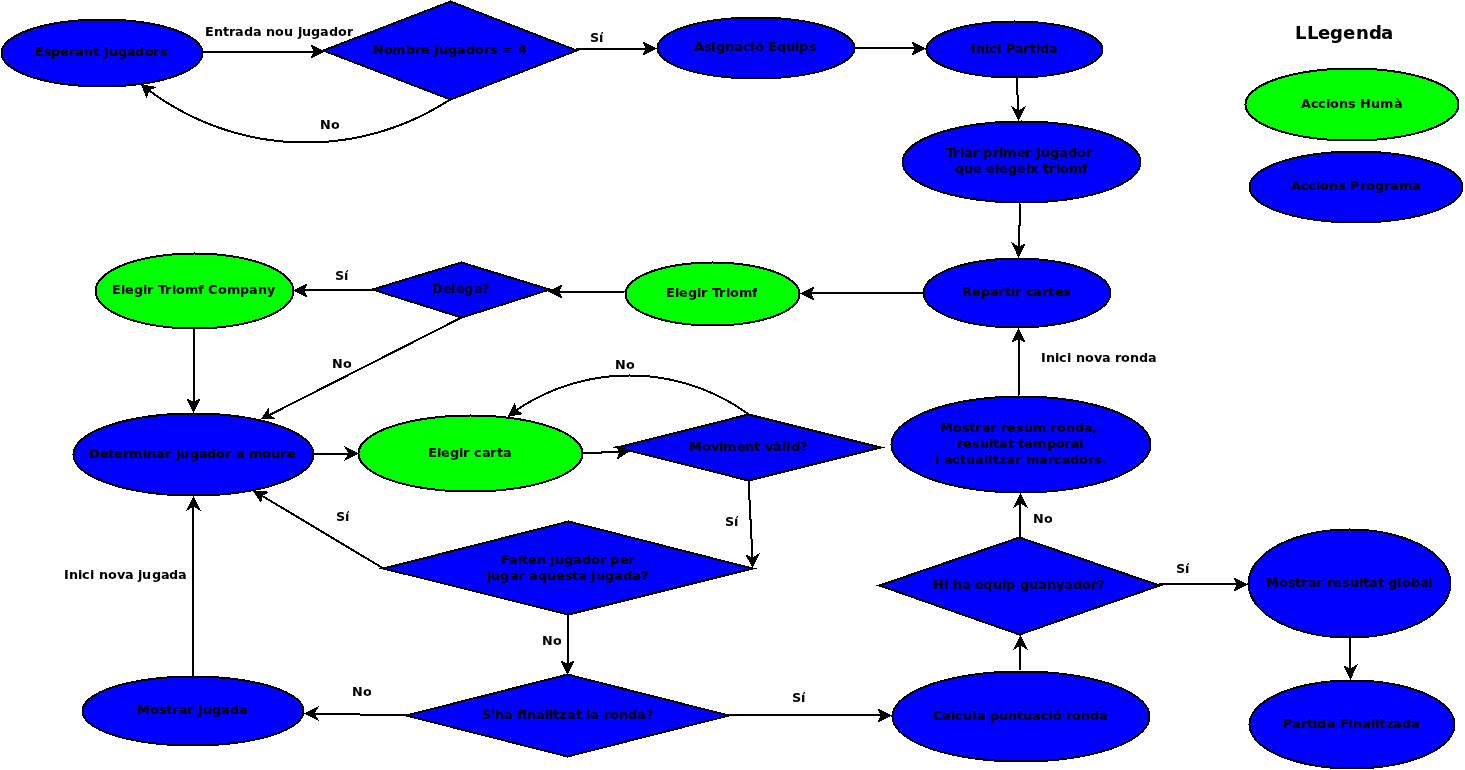
\includegraphics{img/butifarra_workflow.png}
\caption{Flux de treball de la botifarra}
\label{fig:buti-workflow}
\end{figure} 

\newpage

Com es pot observar a la figura \ref{fig:buti-workflow} el servidor s'encarrega de realitzar les següents tasques referents a la botifarra: 

\begin{itemize}
\item{Començar la partida quan ja hi ha cuatre jugadors. }
\item{Repartir de forma aleatoria els jugadors amb dos equips. }
\item{Tirar de forma aleatoria el primer jugador en elegir triomf.}
\item{Repartir les cartes de forma aleatòria entre els diferents jugadors}
\item{Comunicar el triomf elegit a tots els jugadors.}
\item{Comunicar als jugadors si hi ha algun jugador que contrar.}
\item{Determinar el jugador a moure i notificar-lo de que es el seu torn.}
\item{Validar que la carta jugada es la correcta}
\item{Mostrar les cartes de cada jugada.}
\item{Al final de cada ronda mostrar el resultat parcial de la ronda. }
\item{Al final de cada ronda calcular la puntuació de cada equip. En el cas que hi haigi un equip guanyador finalitzar la partida. En el cas que no hi haigi cap jugador guanyador inicial una nova ronda.}
\end{itemize}

Tota la lògica de la butifarra s'ha realitzat a base d'events, es a dir, cada vegada que es produeix un acció que requereix la intervenció del servidor aquest llança un event que té asociada una funció. Aquesta funció es l'encarregada de realitzar tot el procesament i llençar el proxim event en cas de que sigui necesàri.  


\subsubsection{Aleatorietat}

Un punt molt important per a que els jugadors disfrutin de la seva partida de la botifarra és l'aleatorietat del repartiment de les cartes. Per garantir aquesta aleatorietat s'ha implementar l'algorisme de Knuth Fisher Yates\footnote{\url{http://en.wikipedia.org/wiki/Fisher-Yates_shuffle}} que permet la generació d'una permitacuó aleatoria sobre un conjunt finit. En el nostre cás el nostre conjunt finit es correspon amb les 48 cartes de la barralla espanyola utilitzades per jugar a la botifarra. 

Donat un conjunt de nombre de 1 a N, aquest algoritme s'aplica de la següent forma: 
\begin{enumerate}
\item{Escriure els nombre de 1 a N.}
\item{Agafar un nombre aleatori k entre 1 i el nombre d'elements pendents de tractar (inclsiu)}
\item{Contant per la part més baixa, treure el número de la posició k que encara no s'ha tractat i escriurel a un altre lloc}
\item{Repetir el segon pas fins que s'hagin tractat tots els nombres}
\item{El conjunt de nombres que s'han escrit al pas 3 es una permutació aleatòria del conjunt de nombres inicials}
\end{enumerate}

Aquest algorisme te un cost $O(n^2)$ per això s'ha utilitzat la variant de Knuth que permet optimitzar l'alogrisme fins a obtenir un cost de $O(n)$. Aquesta variant el que fa es moure els elements pendents de tractar al final de lla llista. Així l'algorisme es queda expresat de la següent forma: 

\begin{verbatim}
 Per ordenar un conjunt de n elements (indexos 0..n-1):
   Per cada i de n - 1 fins a 1 fer:
        j <- nombre aleatory que compleix que  0 <= j <= i
        cambiar a[j] i a[i]
\end{verbatim}

A més a més per tal de garantir la complerta aleatorietat i evitar posibles resultats iguals aquest algorisme s'aplica 12 vegades. Amb això s'aconsegueix emular el comportament humà al barrejar la baralla de cartes. 

\section{Client}

\subsection{Lògica del client}

\subsection{Visualització de la informació}
